\chapter{Methodology}
\label{chapter4}

In Chapter \ref{chapter4}, we will define and elaborate on the software development methodology that was followed through the different processes of this project. We will also explain other workflows that complemented this methodology such as the usage of version control and a Kanban board for issue tracking and backlogging of features and fixes.

\section{Waterfall}

On the initial planning, the development methodology that was designated to be used through our project was be an iterative or waterfall model \cite{balaji_waterfall_2012}, since it seemed clear that each phase had to be completed before starting the next and no work was planned in parallel. Development would then be organized following the schema in Figure \ref{fig:waterfall} \cite{noauthor__2021}.

\begin{figure}[h]
  \centering
  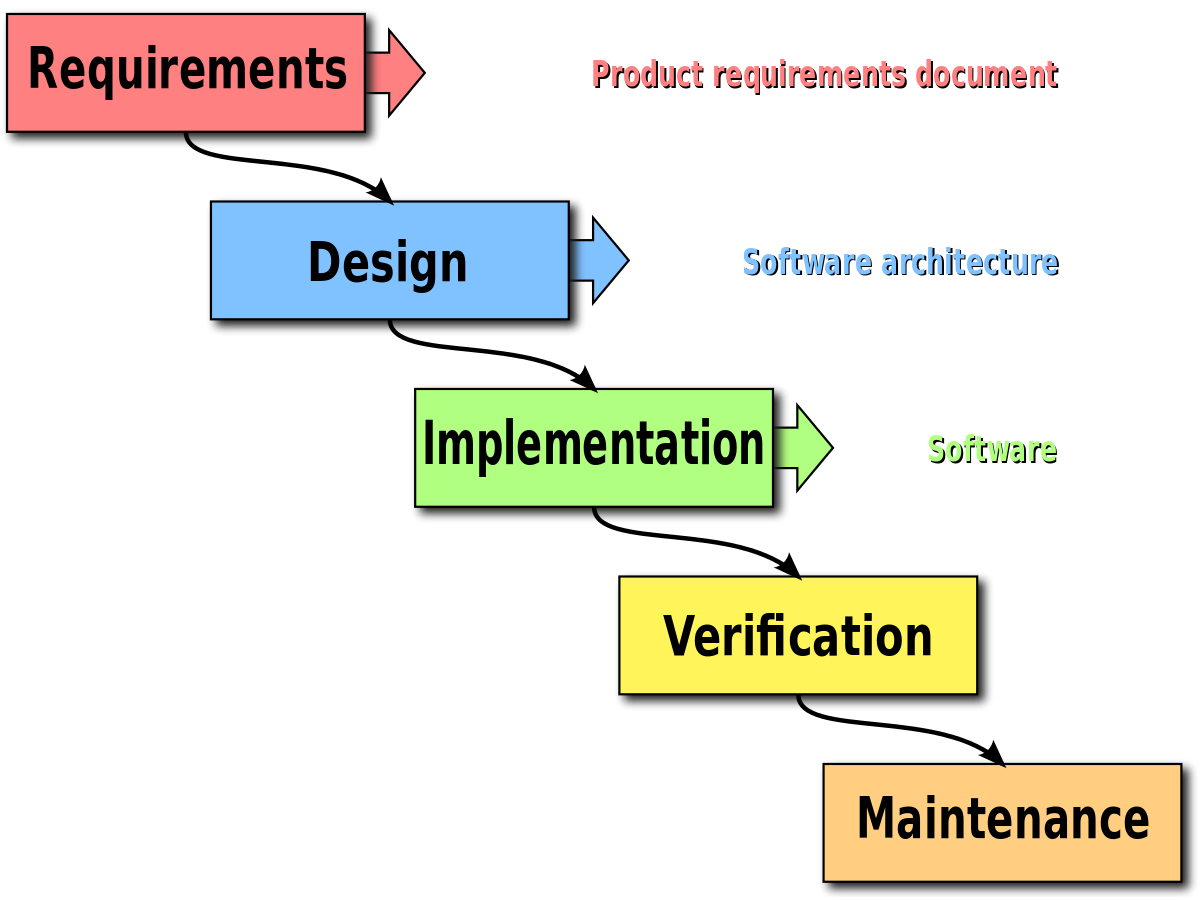
\includegraphics[width=0.6\textwidth]{Figures/waterfall.png}
  \caption{%
    Waterfall methodology base schema
  }
  \label{fig:waterfall}
\end{figure}

However, shortly upon the start of the project, it was clear that this was not the ideal methodology to follow. While the main intention was to complete every stage in a sequential manner, we often found the need to go back to iterate on what had already been completed in order to achieve a better solution.

Therefore, it was decided that as the project was going to be developed by a single person, certain flexibility should be adopted by adding some elements from agile methodologies. In this way elements from \textit{scrum} were quickly incorporated into the workflow, such as periodic meetings with the tutor along with the possible revisions of the requirements.

\section{Scrum}

\textit{Scrum} \cite{noauthor_scrum_2022} is an agile methodology for software development designed for small teams, where the final product is broken into several subobjectives to be completed through several \textit{sprints}. These \textit{sprints} are timed iterations of the final product, each of them taking typically around two weeks to complete. The Figure \ref{fig:scrum} shows the main framework for a \textit{scrum} project. 

\begin{figure}[h]
  \centering
  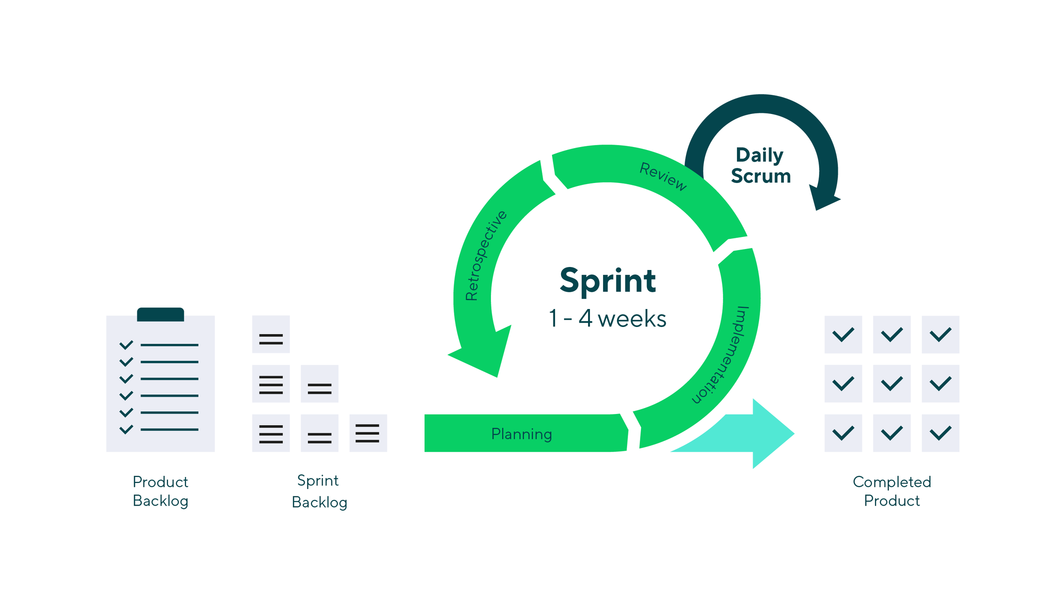
\includegraphics[width=\textwidth]{Figures/scrum.png}
  \caption{%
    Scrum methodology base schema
  }
  \label{fig:scrum}
\end{figure}

We can see each \textit{sprint} is composed of a Sprint Backlog, whose elements are at the same time a subset of objectives taken for a Product Backlog. This Product Backlog is a list containing each and every objective that needs to be materialized in order to compose the finished project. The elements taken from the Product Backlog for each \textit{sprint} are usually chosen considering the best ratio between the time required and the importance or satisfaction for the client.

In the particular case of this project, Sprint Backlogs were not formally defined, as the timezone difference and other incompatibilities made it difficult to have frequent and fixed in time meetings with the Scrum Master (the DFP director in this case) which delimit and determine the contents of each \textit{sprint}.

However, a Product Backlog was established and several deadlines were defined in order to ensure that the development progressed according to the schedule. The most crucial items were selected from the Product Backlog in each iteration according to the criteria of the developer. This Product Backlog was implemented into the workflow by using a Kanban board.

\section{Kanban}

Kanban \cite{noauthor_kanban_2021} is a framework or methodology for software development which is centered around a Kanban board. In a Kanban board, tasks are presented as cards and distributed across several columns, usually representing the possible stages of development for every job. 

In our project, we utilized a Kanban board as an organization tool for keeping track of both issues and proposed features. Using GitHub projects \cite{noauthor_githubcom_2021}, we can automate the board so as to automatically move the tasks as we mark as solved the issues associated. The Kanban board for the project can be seen in Figure \ref{fig:kanban}, and it can also be found in its corresponding GitHub repository\footnote{Available at: \url{github.com/dogudo/tfg}}.

\begin{figure}[h]
  \centering
  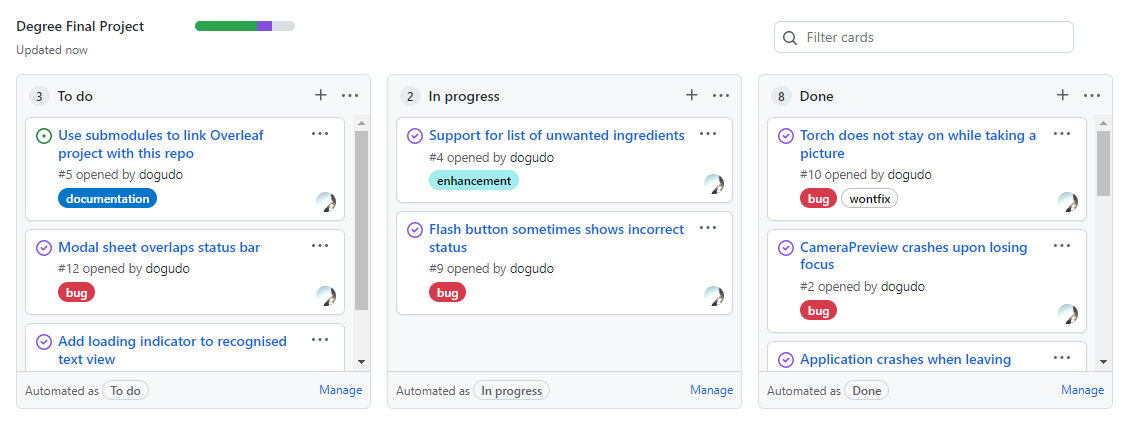
\includegraphics[width=\textwidth]{Figures/kanban_board.png}
  \caption{%
    Kanban board
  }
  \label{fig:kanban}
\end{figure}

The issues that feed the Kanban board are created at the Issues section of the GitHub repository. In this tab we can create entries for any kind of issue or enhancement and associate some tags to them, such as \textit{bug}, \textit{feature}, \textit{documentation}, etc. We can also assign any user to the task (in this case all of the tasks are assigned to the repository owner) and allocate them to different milestones, which can function similar to the \textit{sprints} proposed in \textit{scrum} methodology. The issue tracker view is shown in Figure \ref{fig:issue-tracking}.

\begin{figure}[h]
  \centering
  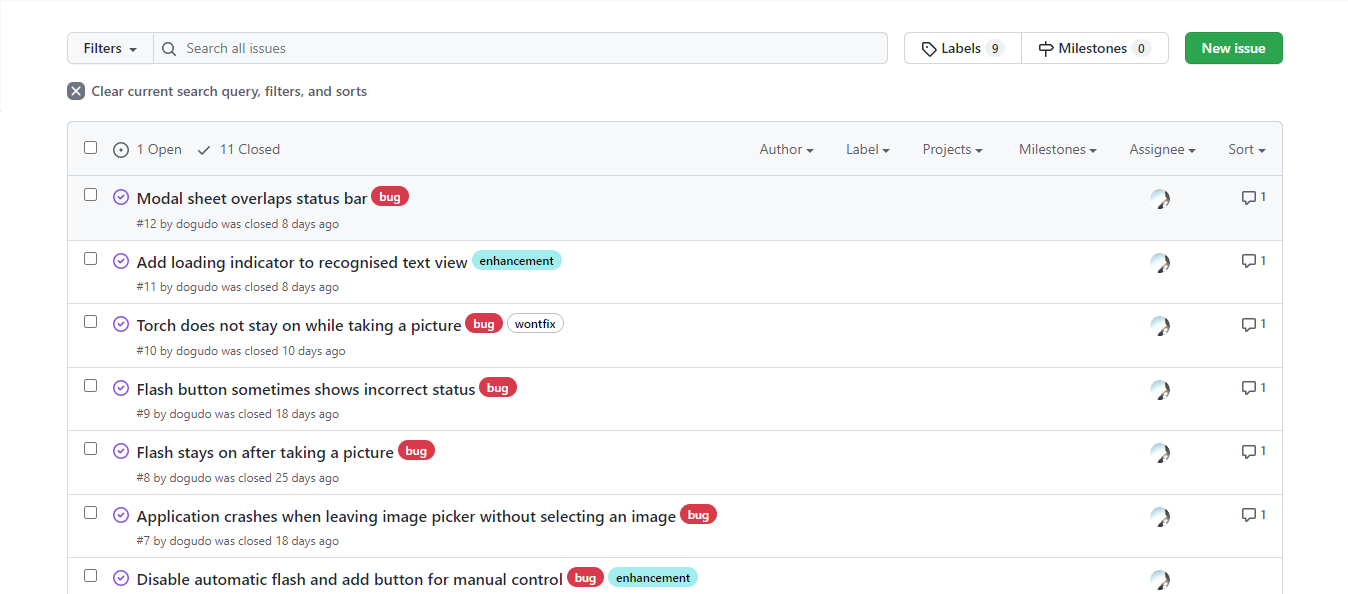
\includegraphics[width=\textwidth]{Figures/issue_tracking.png}
  \caption{%
    Issue tracking
  }
  \label{fig:issue-tracking}
\end{figure}

If we open any of this issues, a timeline view is shown we can add any type of comments to keep reference of the progress being made. Figure \ref{fig:timeline} depicts this timeline view for one of the issues, which has some comments, commits, and a Kanban card associated with it.

\begin{figure}[h]
  \centering
  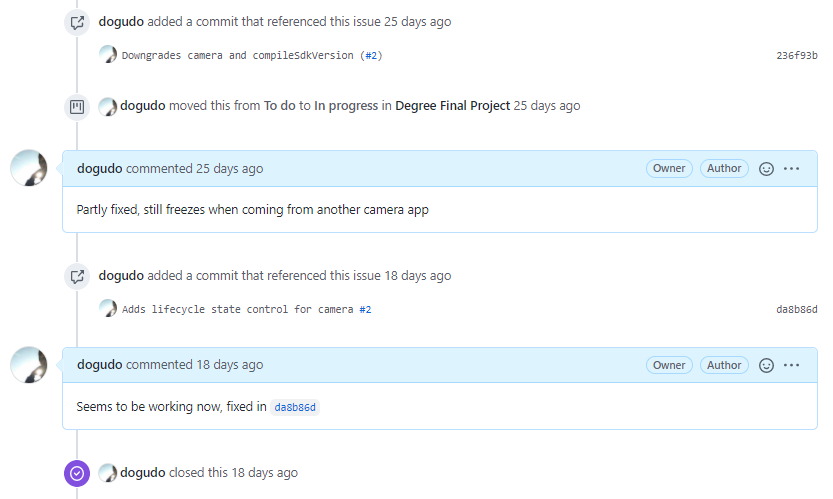
\includegraphics[width=0.8\textwidth]{Figures/issue_timeline.png}
  \caption{%
    Example of timeline view for an issue
  }
  \label{fig:issue-timeline}
\end{figure}

As mentioned before, we can also use the Milestones feature to associate a set of issues with a due date, therefore emulating the \textit{sprints} that characterize the \textit{scrum} methodology. Figure \ref{fig:milestones} shows two of the milestones that were defined for the project.

\begin{figure}[h]
  \centering
  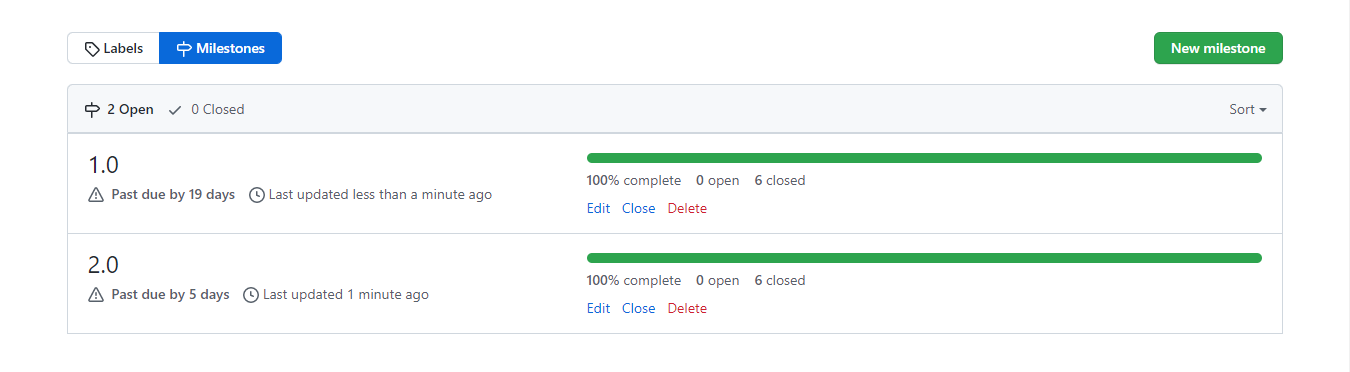
\includegraphics[width=\textwidth]{Figures/milestones.png}
  \caption{%
    Milestones for the project
  }
  \label{fig:milestones}
\end{figure}